% ---------------------------------------------------------------------- %

\documentclass[letterpaper,10pt]{article}



\pagestyle{empty}

\usepackage[table]{xcolor}
\usepackage{color, colortbl}
\usepackage{tabularx}
\usepackage{amssymb}
\usepackage{enumerate}

\definecolor{LightGray}{gray}{0.9}

\usepackage{amsmath}
\usepackage{amscd}
\usepackage{url}

\usepackage{graphicx}


\title{Installing AIMBAT}
\author{Seismo Group}
\date{\today}

\begin{document}
\maketitle

% ************************************************************* %
%                                                               %
%                       MACPORT UPGRADES                        %
%                                                               %
% ************************************************************* %

\section{Macport Problems}

You may run into problems with AIMBAT if your Macport version is not compatible with your operating system version. For example, if you used Macports for OS X 10.8 to install AIMBAT, then upgraded your operating system ot OS X 10.9, you may find that AIMBAT no longer works properly. You will need to upgrade Macports to fix this error.

Do not uninstall MacPorts unless you know what you are doing, uninstalling MacPorts may get rid of other programs you installed using MacPorts. However, if you are sure you want to do so, see here for instructions: \url{https://guide.macports.org/chunked/installing.macports.uninstalling.html}. 

% \begin{figure}[h!]
%   \centering
%   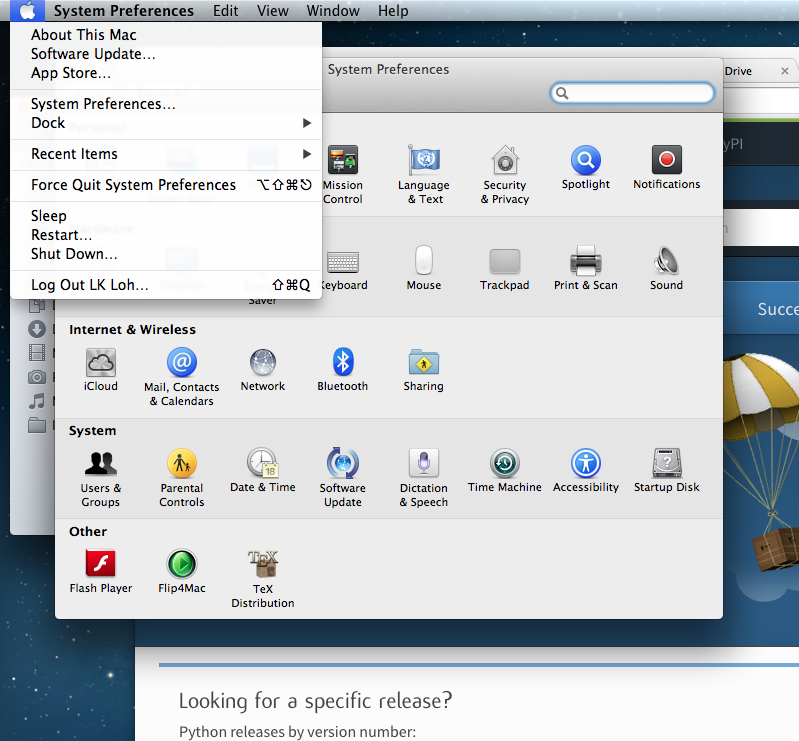
\includegraphics[width=0.5\textwidth]{images/system_preferences}
%   \caption{Console}
%   \label{fig:system_preferences}
% \end{figure}


% ************************************************************* %
%                                                               %
%                       MACPORT UPGRADES                        %
%                                                               %
% ************************************************************* %

% ************************************************************* %
%                                                               %
%                     SETTING THE PYTHON PATH                   %
%                                                               %
% ************************************************************* %

\section{Setting the Python Path to the scripts}

You are asked to add the path to the AIMBAT scripts in your file. To do that, you add them to the \verb".bashrc" file. There are other files you could add it to that work as well, such as the \verb".profile" or \verb".bash_profile" files. You can see the files by opening the terminal and doing \verb"ls -a" to see all the hidden files, and open then by doing \verb"vi .bashrc" in vim, for instance.

To ensure you can open a script, you need to add
\begin{verbatim}
  export PATH=$PATH:<path-to-folder-with-scripts>
  export PYTHONPATH=$PYTHONPATH:<path-to-folder-with-scripts>
\end{verbatim}
to the \verb".bashrc" file. We recommend adding the paths to the \verb".bashrc" file, for reasons listed here: \url{http://stackoverflow.com/questions/415403/whats-the-difference-between-bashrc-bash-profile-and-environment}.
























% ************************************************************* %
%                                                               %
%                     SETTING THE PYTHON PATH                   %
%                                                               %
% ************************************************************* %




% ------------------------------------------------------------------------- %

\end{document}

% --------------------------------- END --------------------------------- %
